\documentclass[letterpaper]{article}

\newcommand{\doctitle}{Lab 8: Microbenchmarks and SIMD Instructions}
\newcommand{\docauthor}{Matthew Duschenes}
\newcommand{\docaffil}{Department of Applied Physics, University of Michigan}

\newcommand{\docheader}{NERS 570 - Lab 8 - \docauthor}
\newcommand{\docfooter}{\docaffil}

% Margins
\usepackage[margin=0.75in,marginparsep=0pt,paperwidth=216mm,paperheight=279mm]{geometry}

% Headers
\usepackage{fancyhdr}
\geometry{headheight=15pt}
\renewcommand{\headrulewidth}{0.4pt}% default is 0.4pt
\renewcommand{\footrulewidth}{0.4pt}% default is 0pt
\geometry{headheight=15pt}
\geometry{headsep=10pt}
\setlength{\skip\footins}{10pt} % gap between text and footer
\fancyhf{}
\fancyhead[R]{\docheader}
\fancyfoot[LE,RO]{\thepage}
\fancyfoot[LO,RE]{\docfooter}

% \makeatletter
% \if@twoside
% \fancyfoot[LE,RO]{\thepage}
% \fancyfoot[LO,RE]{\docfooter}
% \else
% \fancyfoot[R]{\thepage}
% \fancyfoot[L]{\docfooter}
% \fi
% \makeatother
% \fancyhead[R]{\docheader}


% Title
\usepackage{titling}
% \usepackage[affil-it]{authblk}
\usepackage[nodayofweek]{datetime}
\usepackage[super]{nth}

% \newdateformat{monthdayyear}{%
%   \monthname[\THEMONTH]~\THEDAY,~ \THEYEAR}
% \newdateformat{mydate}{\monthname[\THEMONTH] \nth[\THEDAY], \THEYEAR}


% Make Title
\pagestyle{fancy}
% \renewcommand*{\Authfont}{\bfseries}
% \renewcommand*{\Affilfont}{\normalfont\itshape}
\pretitle{\begin{center}\vskip -50pt}%
\title{\large \doctitle}
\posttitle{\end{center}}
\preauthor{\begin{center} \vskip -20pt}
\author{}
\postauthor{\end{center} \vskip -20pt}
\predate{\begin{center} \vskip -20pt}
\date{}%\small{\today}}
\postdate{\end{center} \vskip -20pt}% -42.5pt


% Fonts
\usepackage[singlespacing]{setspace}
\usepackage{dirtytalk}
 
% Math
\usepackage{amsmath}
\usepackage{amssymb}
\usepackage{physics}


% Figures
\usepackage{floatrow}
\usepackage{multicol}
\usepackage{grffile}
\usepackage{caption}
\usepackage{subcaption}
\usepackage{graphicx,xcolor}
\PassOptionsToPackage{export}{adjustbox}

% HypperReferences
\usepackage[pdftex,draft=false]{hyperref}
\hypersetup{
    colorlinks=true,
    linkcolor=black,
    citecolor=black,
    urlcolor=black}
\usepackage{url}

% References
\usepackage[capitalize]{cleveref}


% Code
\usepackage{minted}
\renewcommand\listingscaption{Code}
\floatsetup[listing]{style=Plaintop}    

\crefname{listing}{Code.}{Code}
\newminted{python}{frame=lines,framerule=2pt,float=ht}
\setminted{breaklines,frame=single,framesep=2pt,breakindent=10pt,breakafter={,},breaksymbolleft=}

\newenvironment{longlisting}{\captionsetup{type=listing}}{}
\newcommand{\code}[4]{
% \begin{listing}[ht]
\begin{longlisting}
    \caption{#3}
    \inputminted{#1}{#2}
    \label{code:#4}
\end{longlisting}
% \end{listing}
}


 % Commands
\newcommand{\reals}{\mathbb{R}}
\DeclareMathOperator*{\argmax}{arg\,max}
\DeclareMathOperator*{\argmin}{arg\,min}

\newcommand{\eqtxt}[1]{\overset{#1}=}
\newcommand{\repo}[2]{\href{https://github.com/bkochuna/ners570f20-Lab06/#1/#2}{\##2}}


%%%%%%%%%%%%%%%%%%%%%%%%%%%%%%%%%%%%%%%%%%%%%%%%%%%

%%%%%%%%%%%%%%%%%%%%%%%%%%%%%%%%%%%%%%%%%%%%%%%%%%%
\begin{document}

%%%%%%%%%%%%%%%%%%%%%%%%%%%%%%%%%%%%%%%%%%%%%%%
\maketitle
\pagestyle{fancy}
% \singlespacing

%%%%%%%%%%%%%%%%%%%%%%%%%%%%%%%%%%%%%%%%%%%%%%%%



\section{Membench}
The \textit{membench} programs are run to obtain the following plot in \cref{fig:membench} for the effect of array length and stride length on type of memory access, and time to access. The following script \textit{calc.sh} in the appendix was used to calculate the average processor speed for the $36$ processors on GreatLakes to be 3000 MHz. This speed will be used to calculate the number of processor clock cycles required to access the various types of memory, 
$$\textrm{\# cycles per memory access} = \textrm{clock speed}~\times~\textrm{memory access time}.$$





\begin{figure}[H]
  \centering
  %  trim={<left> <lower> <right> <upper>}
  % \captionsetup{skip=-12pt,format=hang}
  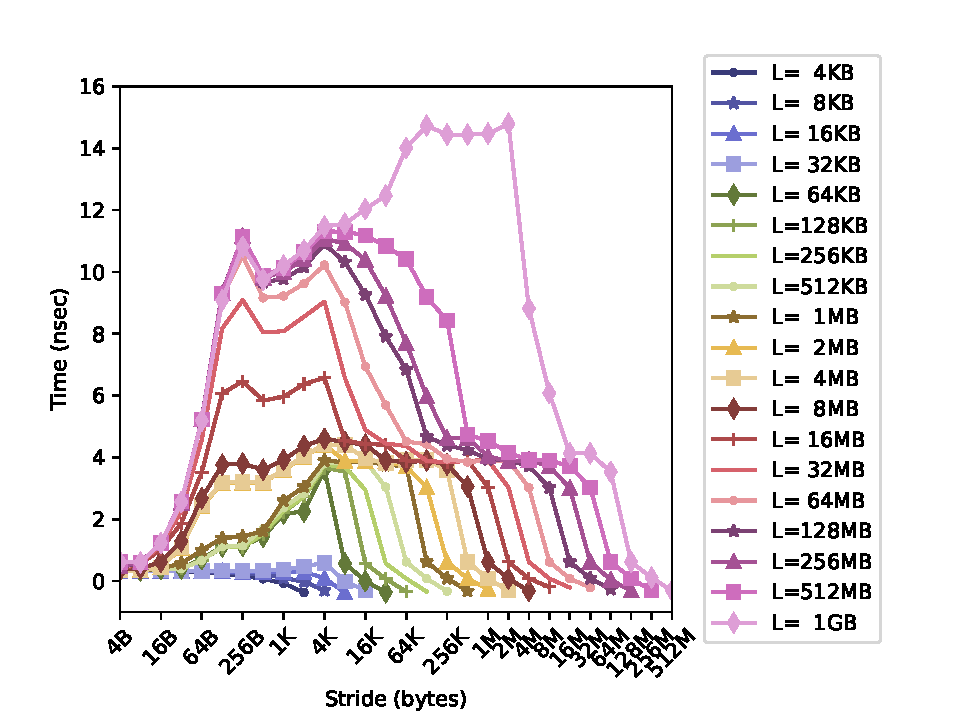
\includegraphics[width=\textwidth]{figures/membench.pdf}
  % \vspace{-8pt}
  \caption{Memory access times for various array sizes and stride lengths}
  \label{fig:membench}
\end{figure}


\section{SIMD Instructions}

\subsection{AVX Support}
\begin{itemize}
	\item The commands used to verify if the current machine/processor supports AVX are:
	$$ \textrm{grep -E \say{avx[\^{}0-9]} /proc/cpuinfo}$$
	and if the current machine/processor supports AVX2 are:
	$$ \textrm{grep -E \say{avx2} /proc/cpuinfo}$$
	These searches will show whether the supported AVX fields are in the flags section of the processor info from /proc/cpuinfo. This command will show all processors (36 $\times$ Intel(R) Xeon(R) Gold 6140 CPU @ 2.30GHz, for GreatLakes compute nodes).
)


\end{itemize}




%%%%%%%%%%%%%%%%%%%%%%%%%%%%%%%%%%%%%%%%%%%%%%%%
\end{document}